%\documentclass[aspectratio=43]{beamer}
\documentclass[t]{beamer}
\usetheme{ffmodern}  %% Themenwahl

\usepackage[ngerman]{babel}
\usepackage[T1]{fontenc}    % richtige Silbentrennung
\usepackage[utf8]{inputenc} % Umlaute etc.!
\usepackage{eurosym}
\usepackage{tikz}
\usepackage{pgffor}
\usepackage{textcomp}
\usepackage{textpos}
\usepackage{tikz}
\usepackage{mathtools}
\usepackage{grid-system}

\usetikzlibrary{arrows,decorations.pathmorphing,backgrounds,fit,positioning,shapes.symbols,chains}

%-----------------
\title{Freifunk Darmstadt}
\author{Freies Funknetz in Darmstadt} % TODO: anderer Untertitel? Bürgernetz?
\date{14. Oktober 2016}
\license{CC-BY-3.0}

\begin{document}

  \maketitle
  
  %-----------------
  \begin{frame}{Was ist Freifunk?}
    \begin{itemize}
      \item Initiative für freie (Funk-)Netze
      \item Offen für jeden, als Nutzer oder Anbieter
      \item Netz in Nutzerhand
      \item Nicht kommerziell
      \item Netzneutral
      \item Krisensichere Kommunikation
    \end{itemize}
  \end{frame}

  %-----------------
  \begin{frame}{Was ist Freifunk?}
    \begin{center}
      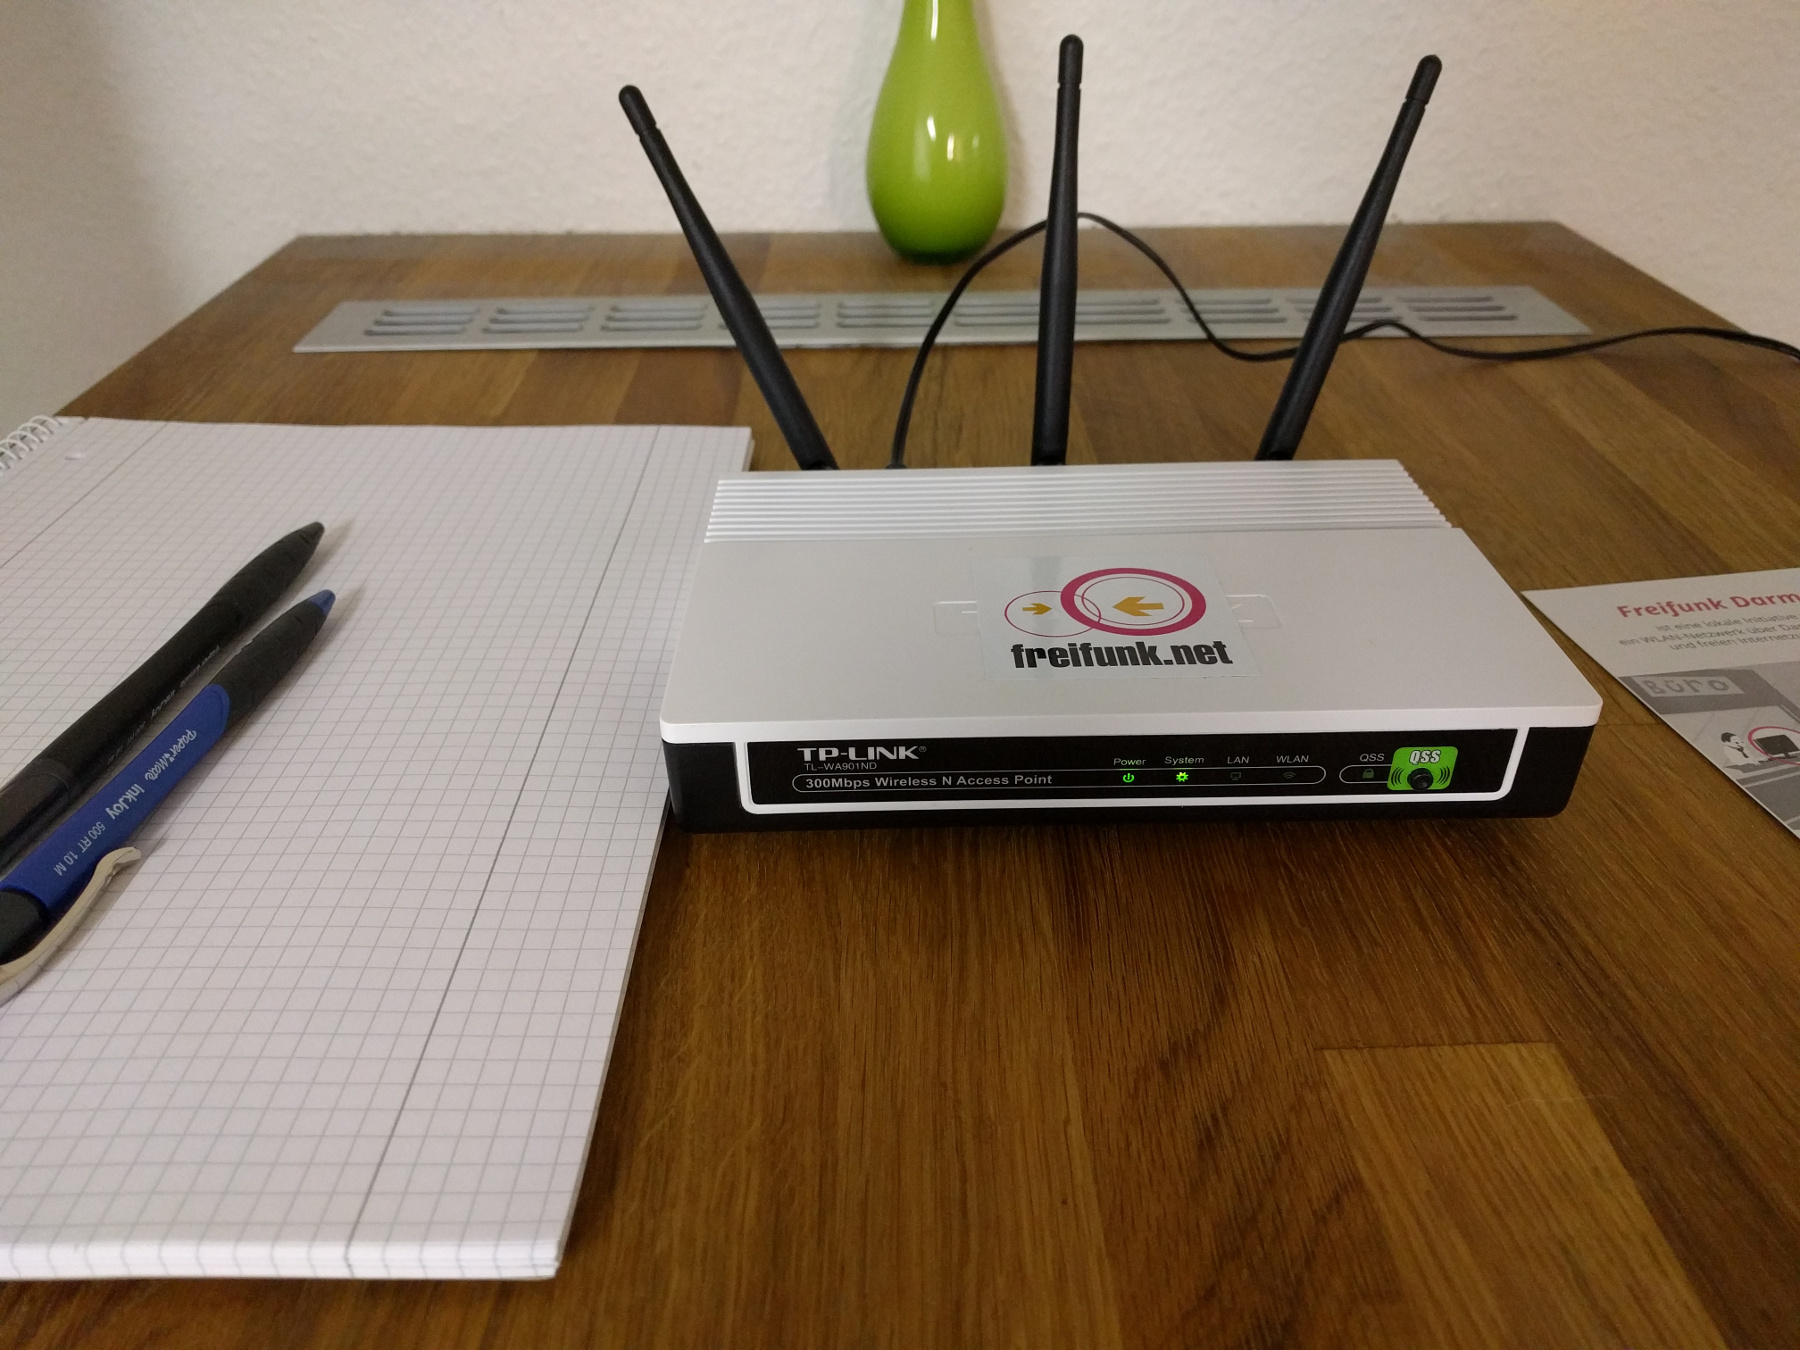
\includegraphics[width=7cm]{images/homerouter}
    \end{center}
  \end{frame}

  %-----------------
  \begin{frame}{Verbreitung}
    \begin{columns}
      \begin{column}{0.6\textwidth}
        \begin{itemize}
          \item Deutschlandweit über  \href{http://freifunk.net/wie-mache-ich-mit/community-finden/}{330 lokale Gruppen}
          \item mehr als 38.000 offene Zugangspunkte
        \end{itemize}
      \end{column}
      \begin{column}{0.4\textwidth}
        \begin{center}
          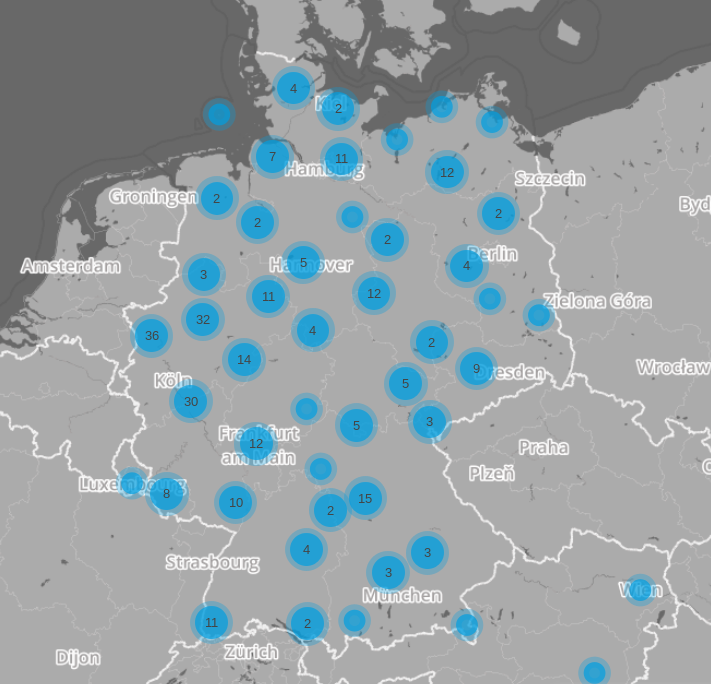
\includegraphics[width=\textwidth]{images/2016-06-01_map-de}
        \end{center}
      \end{column}
    \end{columns}
  \end{frame}
  
  %-----------------
  \begin{frame}{Wie Freifunk Funktioniert}
    \begin{center}
      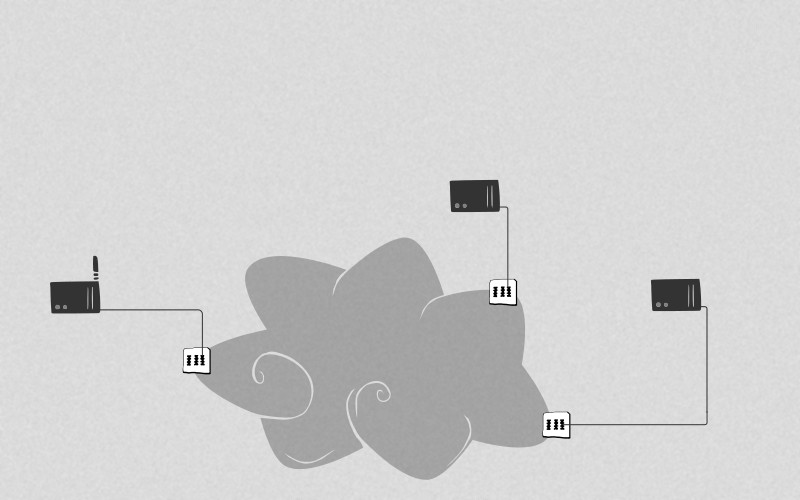
\includegraphics[height=5cm]{images/network_1}\\
      \vspace{1em}
      Geschlossene WLAN-Netze, welche nicht miteinander kommunizieren
      \vspace{1em}
    \end{center}
  \end{frame}

  %-----------------
  \begin{frame}{Mit Freifunk}
    \begin{center}
      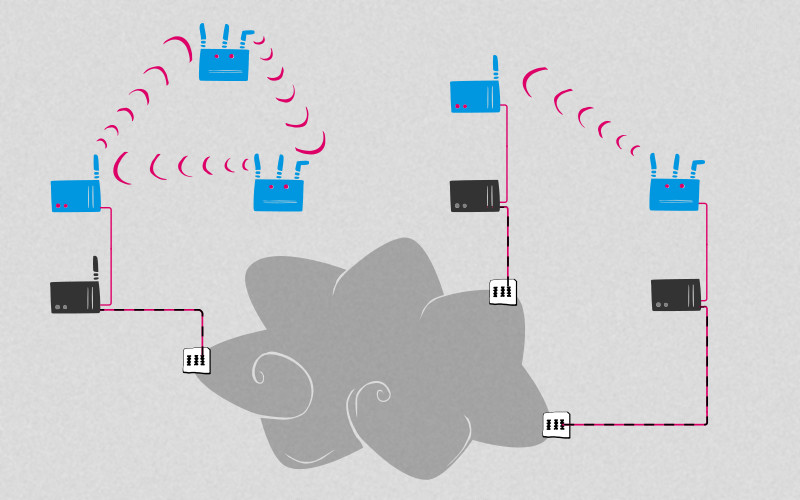
\includegraphics[height=5cm]{images/network_4}\\
      \vspace{1em}
      Freifunk-Knoten spannen ein freies Netz auf
      \vspace{1em}
    \end{center}
  \end{frame}

  %-----------------
  \begin{frame}{Ziele von Freifunk}
    \begin{itemize}
      \item \textbf{Beteiligung der Bevölkerung} an Aufbau und Entwicklung \textbf{dezentraler Netze}
      \item Verständnis von Kommunikationsnetzen fördern $\xRightarrow{}$ \textbf{Bildungsauftrag}
      \item Beteilung an gesellschaftlichen Initiativen, um die \textbf{Verbreitung freier Netze} zu unterstützen
    \end{itemize}
  \end{frame}

  %-----------------
  \begin{frame}{Richtfunknetz}
    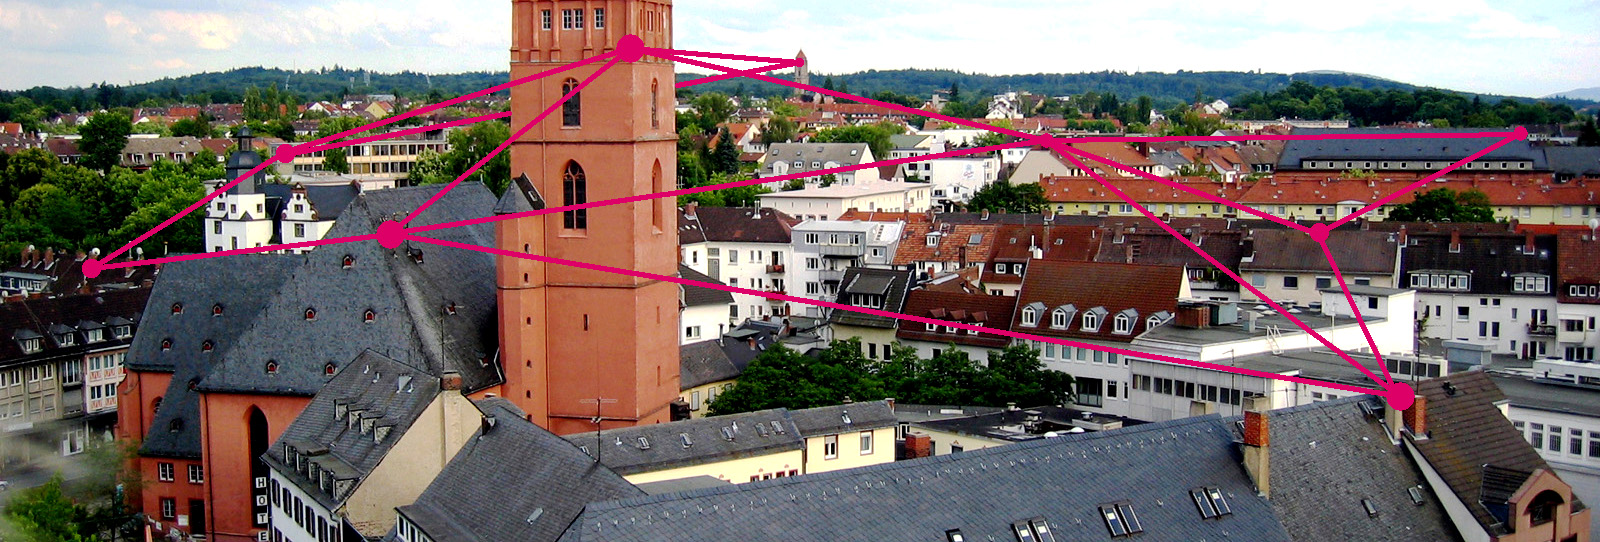
\includegraphics[width=\textwidth]{images/banner-stadtkirche-darmstadt}
    \begin{columns}
      \begin{column}{0.65\textwidth}
        \begin{itemize}
          \item Eigene Infrastruktur
          \begin{itemize}
            \item Redundanz und Lastverteilung
            \item Unabhängig vom Internet
          \end{itemize}
        \end{itemize}
      \end{column}
      \begin{column}{0.25\textwidth}
        \begin{center}
          \vspace{-1.5cm}
          \hspace{-0.75cm}
          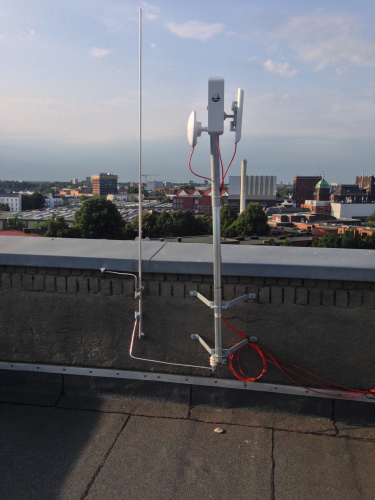
\includegraphics[width=\textwidth]{images/hamburg-richtfunkmast}
        \end{center}
      \end{column}
    \end{columns}
  \end{frame}

  %-----------------
  \begin{frame}{Richtfunknetz}
    \begin{center}
      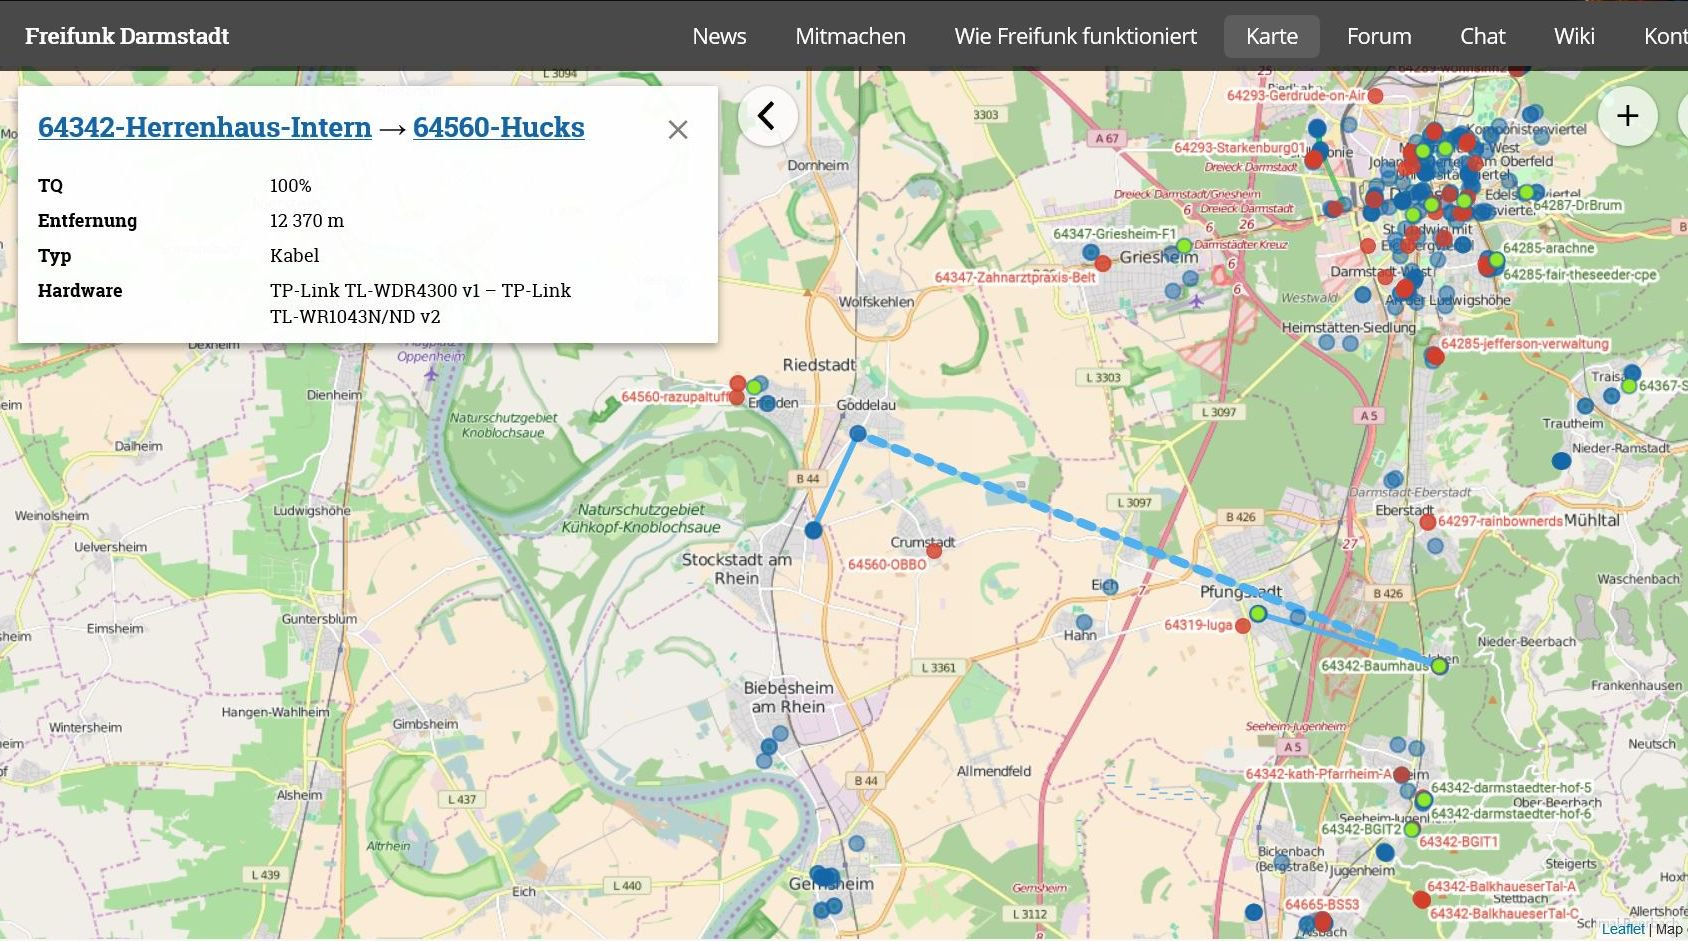
\includegraphics[width=0.95\textwidth]{images/richtfunk_malchen_stockstadt_pfungstadt}
    \end{center}
  \end{frame}

  %-----------------
  \begin{frame}{Kosten}
    \begin{itemize}
      \item Router und Uplink durch Freifunker (Knotenaufsteller)
      \item Hardware je nach Nutzungsart ab 20,- €
      \item Kosten pro Knoten: Ca. 6,- \texteuro\ pro Router und Jahr
    \end{itemize}
  \end{frame}
  
  %-----------------
  \begin{frame}{Kosten}
    \begin{itemize}
      \item Ziel von Freifunk: Kostenlose Teilnahme
      \item Infrastruktur für den Betrieb des Netzes kostet!
      \begin{itemize}
      	\item Betrieb der Internetanbindung, Strom, etc. nur durch Sponsoren möglich
      \end{itemize}
    \end{itemize}
  \end{frame}
  
  %-----------------
  \begin{frame}{Freifunk lebt vom Mitmachen}
    \begin{itemize}
      \item Freifunk ist \textbf{kein Dienstleister}
      \item Netz kann nur durch neue Knotenbetreiber wachsen
      \item Freifunker helfen gerne dabei und \textbf{geben Wissen weiter}
    \end{itemize}
  \end{frame}

  %-----------------
  \begin{frame}{Komm zu Uns!}
    \begin{textblock*}{0cm}(\textwidth-2cm,-2cm)
      \begin{figure}[h]
        \def\svgwidth{2.5cm}
        \input{logo.pdf_tex}
      \end{figure}
    \end{textblock*}
    \begin{itemize}
      \item Online
      \begin{itemize}
        \item Webseite: \href{https://darmstadt.freifunk.net}{darmstadt.freifunk.net}
        \item Forum: \href{https://forum.darmstadt.freifunk.net}{forum.darmstadt.freifunk.net}
        \item Chat: \href{https://chat.darmstadt.freifunk.net}{chat.darmstadt.freiunk.net}
        \item E-Mail: \href{mailto:info@darmstadt.freifunk.net}{info@darmstadt.freifunk.net}
        \end{itemize}
      \item Vor Ort
      \begin{itemize}
      	\item Treffen: Jeden Montag ab 18:30 Uhr
        \item Hackspace des Chaos Darmstadt
        \item Wilhelminenstr. 17, 64283 Darmstadt
      \end{itemize}
    \end{itemize}
  \end{frame}
\end{document}
